\documentclass[journal]{IEEEtran}

\usepackage[nospace,nobreak]{cite}
% http://www.ctan.org/tex-archive/macros/latex/contrib/cite/
\usepackage[pdftex]{graphicx}
\graphicspath{{./img/}}
\DeclareGraphicsExtensions{.pdf,.jpeg,.png}
\usepackage{algorithmicx}
% http://www.ctan.org/tex-archive/macros/latex/contrib/algorithmicx/
\usepackage{array}
% http://www.ctan.org/tex-archive/macros/latex/required/tools/
\usepackage{mdwtab}
% http://www.ctan.org/tex-archive/macros/latex/contrib/mdwtools/
\usepackage{eqparbox}
% http://www.ctan.org/tex-archive/macros/latex/contrib/eqparbox/
\usepackage[caption=false,font=footnotesize]{subfig}
% http://www.ctan.org/tex-archive/macros/latex/contrib/subfig/
\usepackage{fixltx2e}
% http://www.ctan.org/tex-archive/macros/latex/base/
\usepackage{stfloats}
% http://www.ctan.org/tex-archive/macros/latex/contrib/sttools/
\usepackage{url}
% http://www.ctan.org/tex-archive/macros/latex/contrib/misc/

% correct bad hyphenation here
\hyphenation{op-tical net-works semi-conduc-tor}


\begin{document}

\title{WWW-Graphics-Module for Mixed-Reality-System}

\author{Hannes~Eilers,~\textit{Master-student,~Chairman~student~group~NorthernStars,~UAS-Kiel,}
Eike~Petersen,~\textit{Master-student,~FH-Kiel}}

% The paper headers
\markboth{Advanced JavaScript project paper, January~2014}%
{Shell \MakeLowercase{\textit{et al.}}: WWW-Graphics-Module for Mixed-Reality-System}

\maketitle

\begin{abstract}
	Warum? Was? Wie? (Max 200 W)
\end{abstract}
\begin{IEEEkeywords}
mixed-reality, javascript, server, client, paper.
\end{IEEEkeywords}

\section{Introduction}

\IEEEPARstart{T}{he}
Mixed-Reality is a robocup soccer league that uses hardware and software
simulation to develop artificial intelligences for robots. The system used for
playing in competitions all over the world\cite{gerndt-case-study} uses a
horizontal screen on which a soccer field with field lines, goals and a ball is
simulated. On this screen real robots with quadratic dimensions for each side of
nearly 2,5cm move. A game server uses a vision system above the screen for
tracking the robots and generating a world-model that includes positions of all
robots as well as simulated objects like goals or important positions on the
field. By using an infrared transmitter the server sends commands to the
robots(Figure~\ref{fig:mr_system}).\\
\begin{figure}[!t]
    \centering
    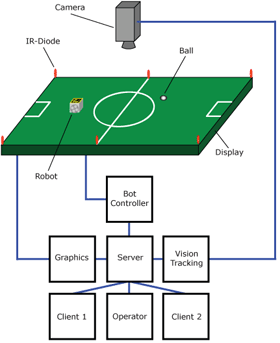
\includegraphics[width=0.3\textwidth]{mr_system.png}
    \caption{\textbf{Mixed-Reality system:} The simulated soccer field is
    controled by a game server that uses several other modules for access to the
    robots, displaying the field or interacting with human operator or
    artifical intelligences}
    \label{fig:mr_system}
\end{figure}
For each robot an artificial intelligence can connect to the game server to
control the movement and actions of the robot. The game-server sends the
world-model to this artificial intelligence, so that it can react to changes on the field.\\
The Mixed-Reality system is module based and uses different modules to track and
control the robots or to display the field on the screen.\\
During a competition teams of artificial intelligences connect to the game
server using a local network to control their designated robots and play matches
against each other in realtime\cite{mr-web-northernstars}, while observers can
watch the game live from the sidelines.

\subsection{Project definition (Was machen wir?)}
The projects goal is to bring the local mixed-reality-games to an audience
everywhere in the world (Figure~\ref{fig:proj_goal}) so that it is possible to
observe matches or even play against each other without being present at the
Mixed-Reality systems location. All that is needed is a device with a HTML5
compliant Browser and an internet-connection with a bit-rate of at least 10-kbit/s downstream.
\begin{figure}[!t]
    \centering
    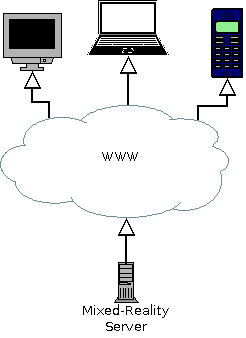
\includegraphics[width=0.3\textwidth]{project-target.png}
    \caption{\textbf{Project goal:} In the 1st~stage we just wanted to bring the mixed-reality-games easily and reliably to end-users on all kinds of devices.}
    \label{fig:proj_goal}
\end{figure}
\subsection{Design (Wie sieht es aus?)}
As in Figure~\ref{fig:proj_design} shown, the web-server is capable to establish
a connection to any Mixed-Reality game-server and game over UDP. This connection
is interchangeable an internal game representation, that converts the incoming
XML to JSON and verifies it, manages the listening clients and encapsulates
needed administrative functions. The verified JSON is sent over websockets at a
fixed interval to the clients, that checks the recieved JSON data for drawable
objects. The objects are drawn using the 2D context of a HTML5
canvas\cite{w3c-canvas}.\\
The client offers forms for login an connecting to a new game, wich is only
nessesary to connect to a new game. Watching a game is open to a non-resitricted
audience.
\begin{figure}[!t]
    \centering
    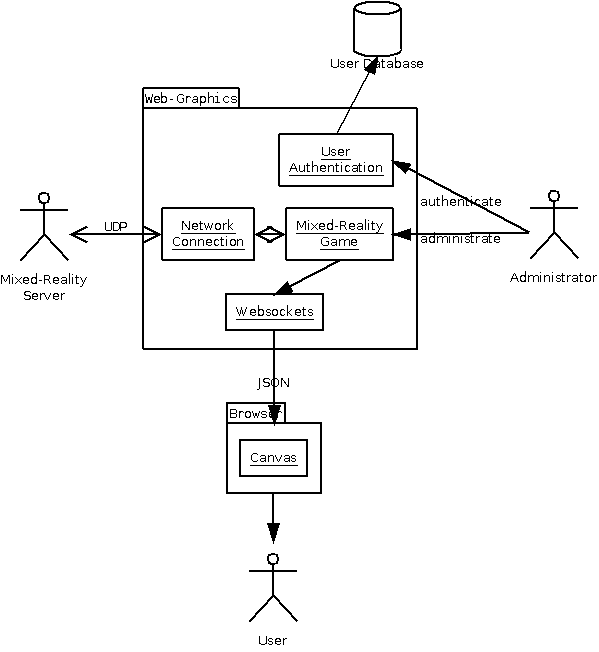
\includegraphics[width=0.3\textwidth]{design.png}
    \caption{\textbf{Project design:} As seen the concept has two parts: the server for connecting to the mixed-reality system and reciving and sending the gamedata to the clients and the client who interprets the data and displays it in a human readable and enjoyable format.}
    \label{fig:proj_design}
\end{figure}
\subsection{Implementation(Wie ist es aufgebaut?)}
\subsubsection{Server}
The design for the server is implemented as a proof-of-concept on the
server-framework Node.js\cite{Node.js} with most of the needed configuration and
essentials implemented with the middle-ware express~\cite{express}, such as
session-management, URL-routing and serving of static files. The Website is
constructed through templates with the template-engine jade\cite{jade} and also served through express.\\
The user-persistence is handled by an sqlite-database with
sqlite3\cite{sqlite3}, because of its convenience to setup and redesign in a
agile software development environment\cite{agile_devel} and the ease of
conversion to a better setup when the project reaches maturity.\\
The communication besides http is managed by
websocket.io\cite{websocket.io}\cite{smash_node.js}, an extension to express.\\
To decode the incoming XML xml2js~\cite{xml2js} is used and to build an easy to
manage and debug system extensive logging is done with log4js\cite{log4js} an
conversion of the Java logging package log4j2\cite{log4j2}.\\
All the modules written for the server use the functional inheritance/creation
pattern\cite{js_goodparts} to create private and secure objects. Every time an
object is needed only once, it is created as a singleton with
closure\cite{js_designpattern} to avoid misuse and implementation errors. The
communication between the mixed-reality-game representation and the connected
websockets is implemented with a simplified observer
pattern\cite{js_designpattern}.\\[3mm]
\subsubsection{Client}
The client side web templates using CSS3\cite{w3c-css3} to specifiy the
user interfaces design, generated from the HTML tags using the jade template
engine. It includes a hidden overlaying login form, thats visibilty is
accessable through an portable javascript function and used for login into webservers administration page.\\
The CSS3 design also resets the browser based drawing styles for common HTML5
tags to define a common design of the clients webpage on different browser
versions. So a unique design for forms or list-like items can be guaranteed.\\
For drawing graphical objects from the recieved JSON data a 2D context of a
HTML5 canvas obejct is used. Everytime new data recieved from the server the
canvas is cleared and the new data is drawn on it. A set of javascript functions
allows context independend drawing of complex objects like rectangles, circles,
dots or robot markers. So a RICH client\cite{rich-client} functkionality for
different mixed-reality szenarios and applications is offered. However currently only
drawing of soccer szenarios is implemented.\\
For drawing simple objects like  rectangles or circles the build in canvas
context instructions\cite{w3c-canvas} are used. For drawing the robots marker a
more complex drawing is implemented, because the marker consists of a image
representing its current position and team color and also a text showing
information about the internal identification number of the robots and its name.
So the client uses a reusable HTMl image object\cite{w3c-image} that is drawn on
the canvas. After that the drawn image is no longer accessable and the image
objetc can be resused for drawing an image again. Using this the bclient doesn't
have to wait before drawing until the image object is loaded through the
browser. The text for the robots information is added to the webpage document as
a html tag with unique id, inside a hidden supsection of the documents
structure. So the text position an orientation can be set using CSS3. This is
nessesary because drawing the text directly on the canvas needs to much
performance for smooth animations of the robot markers.
\section{Conclusion}
The project and the creation of the proof-of-concept have been a success, even
while we where not able to bring mixed-reality to mobile users with smart-phones, because of the spotty HTML5 compliance, we achieved all others of our 1st~stage goals.\\
Even in lieu of this more work is needed to develop the proof-of-concept
further, to be easily and reliably used in the mixed-reality-system. Sorely needed is a rigorous easy  and automatic testing of all components and their implementation, witch has been neglected because of time- and manpower-constraints. Also should we implement all of our 2nd~stage goals, like replays of games, game-chat between spectators and a secure and robust account management with tie-ins to social media. Also when HTML5 will be fully implemented on all mobile devices, we can develop the mobile page.
\section*{Acknowledgment}
The authors would like to thank the Unisversity of Applied Sciences Kiel for use
of their location and rooms, the robotics group NorthernStars,
\url{www.northern-stars.de}, for supporting and helping us on the edges of the project and Prof. Manzke for letting us skirt his regulations, so that we could build something that we can use and develop further for the NorthernStars.\\
Our source-code lies at \url{https://github.com/NorthernStars/MR-Web-Graphics} and everyone who want to use or every develop it further is heartily encouraged to do so.

\begin{thebibliography}{1}

\bibitem{gerndt-case-study}
R. Gerndt, M. Bohnen, R. da Silva Guerra, M. Asada, \emph{The Engineering of
Mixed Reality Systems Human-Computer Interaction Series, Chapter 20: The RoboCup
Mixed Reality League – A Case Study}, 1st~ed. Springer 2010
\bibitem{mr-web-northernstars}
NorthernStars, \emph{Mixed-Reality},
\url{http://northernstars-wiki.wikidot.com/robocup:mixed-reality}
\bibitem{w3c-canvas}
W3C, \emph{HTML Canvas 2D Context}, \url{http://www.w3.org/TR/2dcontext/}
\bibitem{w3c-css3}
W3C, \emph{Introduction to CSS3},
\url{http://www.w3.org/TR/2001/WD-css3-roadmap-20010523/}
\bititem{rich-client}
Wikipedia Foundations,~Inc., \emph{Rich client platform},
\url{https://en.wikipedia.org/wiki/Rich_client_platform}
\bibitem{w3c-image}
W3C, \emph{Objects, Images, and Applets},
\url{http://www.w3.org/TR/REC-html40/struct/objects.html#h-13.1}
\bibitem{Node.js}
Joyent,~Inc, \emph{Node.js}, \url{http://nodejs.org/}.
\bibitem{express}
expressjs.com, \emph{express web~application~framework~for~node}, \url{http://expressjs.com/}.
\bibitem{jade}
jade-lang.com, \emph{jade Node~Template~Engine}, \url{http://jade-lang.com/}.
\bibitem{sqlite3}
MapBox, \emph{node-sqlite3 - Asynchronous, non-blocking SQLite3 bindings for Node.js}, \url{https://github.com/mapbox/node-sqlite3}.
\bibitem{agile_devel}
K.~Beck, \emph{Extreme~programming~eXplained : embrace~change}, 2nd~ed. Addison-Wesley, 2005.
\bibitem{websocket.io}
G.~Rauch, \emph{websocket.io}, \url{https://npmjs.org/package/websocket.io}.
\bibitem{smash_node.js}
G.~Rauch, \emph{SMASHING~Node.js JavaScript~Everywhere}, 1st~ed. WILEY, 2012.
\bibitem{xml2js}
Leonidas-from-XIV, \emph{node-xml2js}, \url{https://github.com/Leonidas-from-XIV/node-xml2js}.
\bibitem{log4js}
nomiddlename, \emph{log4js-node}, \url{https://github.com/nomiddlename/log4js-node}.
\bibitem{log4j2}
Apache Software Foundation, \emph{Apache Log4j 2}, \url{http://logging.apache.org/log4j/2.x/index.html}.
\bibitem{js_goodparts}
D.~Crockford, \emph{JavaScript: The Good Parts}, 1st~ed. O'Reilly, 2008.
\bibitem{js_designpattern}
Data & Object Factory, \emph{JavaScript + jQuery Design Pattern Framework 2013}, Data & Object Factory, LLC, 2013.

\end{thebibliography}

\end{document}


